\chapter{Gaussian Processes and Synthetic Likelihoods}

If the distribution of $\D(\btheta)$ was known for all $\btheta,$ then the need
to sample from the model within Algorithm
\ref{alg:abc} would be redundant since $\D(\btheta)$ could be sampled
directly. Moreover, the probability of drawing and accepting a sample
using this algorithm becomes
$\Pr(\btheta)\Pr(\D(\btheta) < \epsilon | \btheta).$ Comparing
this to Bayes' theorem, we can see that $\Pr(\D(\btheta) < \epsilon | \btheta)$
plays the role of the likelihood. Therefore,
$L(\btheta) := \Pr(\D(\btheta) < \epsilon | \btheta)$
is an approximation of $\L(\btheta)$ (up to some proportionality constant).
In reality, we do not know the distribution of $\D(\btheta)$ for all
$\btheta,$ but we consider methods to construct
an approximation $\hat{L}$ of $L,$ which we call the synthetic likelihood.
The approximation considered is achieved by modelling
$\D(\btheta)$ using a surrogate model, which we introduce in this chapter.

\section{Gaussian Processes}

For $\btheta$ and $\btheta^\prime$ that are close to each other,
the distribution of $\D(\btheta)$ will be similar to the distribution of
$\D(\btheta^\prime).$ Therefore sampling from $\D(\btheta)$ gives information
about the distribution of $\D(\btheta^\prime)$ for $\btheta,$
$\btheta^\prime$ close. A reasonable assumption could be that
$\E(\D(\btheta_1)), \E(\D(\btheta_2)), \dots, \E(\D(\btheta_n))$ are
multivariate
normally distributed with $\cov(E(\D(\btheta_1)), E(\D(\btheta_2)))$ large for
$\btheta_1, \btheta_2$ close, and small for $\btheta_1, \btheta_2$ far apart,
so that $\cov(E(\D(\btheta_1)), E(\D(\btheta_2)))$ is a function of $\btheta_1$
and $\btheta_2.$
Formally, we treat $\E(\D(\beta))$ as a realisation of a Gaussian process.

\begin{definition}[Gaussian Process]\label{def:gp}
    A collection of random variables $\{f(x)\}_{x\in\mathcal{X}}$
    (where $x$ may be a vector) is a \bemph{Gaussian process} if any finite
    subset of the collection of random variables is multivariate normal
    distributed. That is, there is a function $m:\mathcal{X}\to\R$ and
    symmetric kernel $k:\mathcal{X}\times\mathcal{X}\to \R$ such that for all
    finite sets
    $\bx :=\{x_1, x_2, \dots, x_n\} \subset \mathcal{J},$ with
    $f(\bx) := [f(x_1), f(x_2), \dots, f(x_n)]^T$
    $$f(\bx) \sim
        \MVN\left(\begin{bmatrix}
            m(x_1) \\ m(x_2)\\ \vdots\\ m(x_n)
        \end{bmatrix},\, \mathbf{K} = \begin{bmatrix}
            k(x_1, x_1) & k(x_1, x_2) & \dots  & k(x_1, x_n) \\
            k(x_2, x_1) & \ddots      &        & \vdots      \\
            \vdots      &             & \ddots & \vdots      \\
            k(x_n, x_1) & \cdots      & \cdots & k(x_n, x_n)
        \end{bmatrix}\right).$$
\end{definition}

\begin{definition}[Mean Function and Covariance Kernel]\label{def:mean_kernel}
    The \bemph{mean function} and \bemph{covariance kernel} are
    $$m(x_i) := \E\left[f(x_i)\right]$$ and
    $$k(x_{i}, x_{i^\prime}) := \cov\left(f(x_i), f(x_{i^\prime})\right).$$
\end{definition}

Gaussian processes are simultaneously realised over the whole space
$\mathcal{X}$ (for example $\R^d$) and are hence collections of
(uncountably infinite)
random variables. However, the covariance function $k$ is always constructed
such that
$\corr(x, x^\prime) \to 1$ as $||x - x^\prime||\to 0.$
This induces a form of continuity in $x$ called mean square continuity which
is defined in Definition \ref{def:MSC}
The most famous example of a Gaussian process is Brownian motion.

\begin{definition}[Brownian Motion]
    $B(t):\R^+ \to \R$ is a \bemph{Brownian motion} on $\R$ if\begin{enumerate}
        \item $B(0) = 0$ almost surely
        \item $B(t_0), B(t_1) - B(t_0), \dots, B(t_n - t_{n-1})$ are
              independent for all $t_0<t_1<t_2<\dots<t_n$
        \item $B(t + s) - B(t)\sim N(0, s)$ for $s, t \geq 0$
        \item $B(t)$ is continuous almost surely for $t>0.$
    \end{enumerate}
\end{definition}

Brownian motion has zero mean, and covariance kernel $k(s, t) = \min(s, t),$ which
implies that $\corr(B_s, B_t) = \frac{\min(s, t)}{\sqrt{st}}.$ This is close to
$1$ as $s$ is close to $t,$ however as $|s-t|\to\infty,$
$\corr(B_s, B_t) \to 0.$

Gaussian processes can be considered as giving a probability distribution to
functions $f\in\mathcal{F},$ where $\mathcal{F}$ is a class of functions.
The properties of the class of functions
$\mathcal{F}$ depend on the covariance kernel $k.$ Different $k$ result
in very different functions. One such property to consider is the smoothness of
the functions, which we describe by mean square differentiability.

\begin{definition}[Mean Square Continuous]\label{def:MSC}
    A function $f:\R^d\to\R$ is \bemph{mean square continuous} at $\bx$
    in the $i$th direction at $\bx$ if
    $\E(|f(\bx + h\mathbf{e}_i) - f(\bx)|^2)\to 0$ as $|h|\to 0,$
    where $\mathbf{e}_i$ is the unit vector with a 1 in the $i$th coordinate.
\end{definition}

\begin{definition}[Mean Square Differentiable]
    A function $f:\R^d\to\R$ is \bemph{mean square differentiable} at
    $\bx$ in the $i$th direction with derivative
    $\frac{\partial f(\bx)}{\partial x_i}$ if
    $$
        \E\left[
            \left|
            \frac{f(\bx + h\mathbf{e}_i) - f(\bx)}{h}
            - \frac{\partial f(\bx)}{\partial x_i}
            \right|^2
            \right]\to 0
    $$ as $|h|\to 0,$ where $\mathbf{e}_i$ is the unit vector in the direction
    of the $i$th coordinate.
\end{definition}

The concept of mean square differentiability and continuity are analogous to
differentiability and continuity in the non-random function case.

\begin{theorem}
    Brownian motion is mean square continuous, but not mean square
    differentiable.
\end{theorem}
\begin{proof}
    $(B_{t + h} - B_t)^2 \sim (\sqrt{|h|}Z)^2$ where $Z\sim N(0,1).$ Therefore
    $(B_{t + h} - B_t)^2 \sim |h|\chi_1^2 \to 0$ almost surely as $|h|\to 0,$
    hence $\E[(B_{t + h} - B_t)^2] = 0,$ and so Brownian motion is
    mean square continuous. Since
    $\frac{B_{t + h} - B_t}{h} \sim N(0, 1/|h|),$ $\frac{B_{t + h} - B_t}{h}$
    does not converge to any valid probability distribution as $|h| \to 0,$ as
    the variance approaches $+\infty,$ and so Brownian motion is not
    mean square differentiable.
\end{proof}

\subsection*{Kernels}

\subsubsection*{Mat\'{e}rn Kernel Family}

Since we are motivated to consider $\E(\D(\btheta))$ as a realisation of a
Gaussian process, we consider some common choices of kernel function and their
effect on the Gaussian process realisations. The two most common families of
kernel functions are the squared exponential
and Mat\'ern families \parencite{rasmussen_gaussian_2008}.
The Mat\'ern kernel explicitly allows for adjustment of function
smoothness through a hyperparameter $\nu.$

\begin{definition}[Mat\'ern Kernel]
    The \bemph{Mat\'ern kernel} is covariance kernel function of the form
    $$k_\nu(x, x^\prime)
        = \sigma^2_k \frac{2^{1 - \nu}}{\Gamma(\nu)}
        \left(\frac{\sqrt{2\nu}||x - x^\prime||}{\ell}\right)^\nu
        K_\nu\left(-\frac{\sqrt{2\nu}||x - x^\prime||}{\ell}\right),$$
    where $K_\nu$ is a modified Bessel function
    (defined in \cite[374]{abramowitz_handbook_2013}). $\nu, \ell,$ and
    $\sigma_k$ are hyperparameters.
\end{definition}

\begin{figure}[htbp]
    \centering
    \begin{subfigure}[b]{0.5\textwidth}
        \centering
        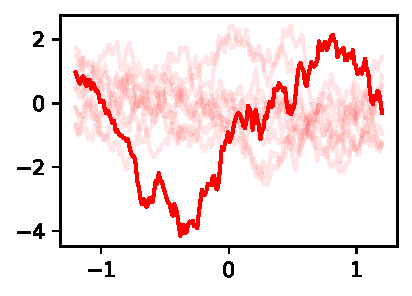
\includegraphics[width=\textwidth]{maternonehalf_kernel.pdf}
        \subcaption{Mat\'ern 1/2 Kernel}
        \label{fig:mat_one_half}
    \end{subfigure}%
    \hfill%
    \begin{subfigure}[b]{0.5\textwidth}
        \centering
        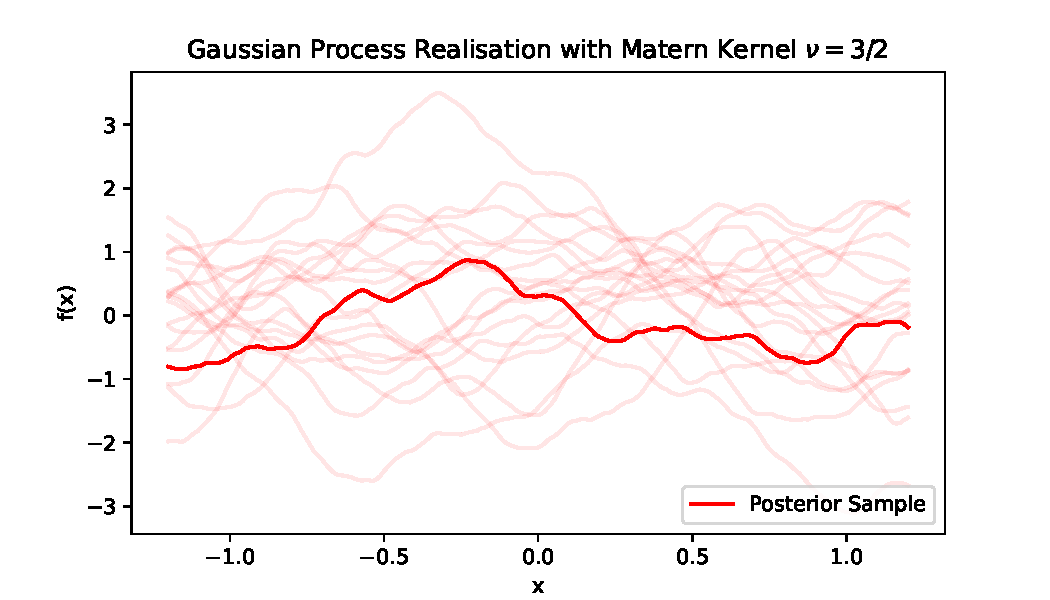
\includegraphics[width=\textwidth]{maternthreehalves_kernel.pdf}
        \subcaption{Mat\'ern 3/2 Kernel}
        \label{fig:mat_three_halves}
    \end{subfigure}
    \begin{subfigure}[b]{0.5\textwidth}
        \centering
        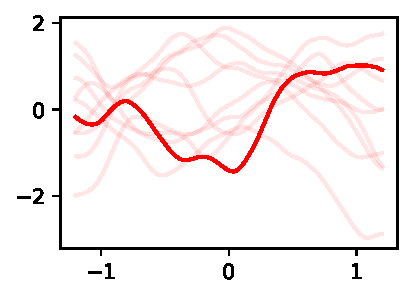
\includegraphics[width=\textwidth]{maternfivehalves_kernel.pdf}
        \subcaption{Mat\'ern 5/2 Kernel}
        \label{fig:mat_five_halves}
    \end{subfigure}%
    \hfill%
    \begin{subfigure}[b]{0.5\textwidth}
        \centering
        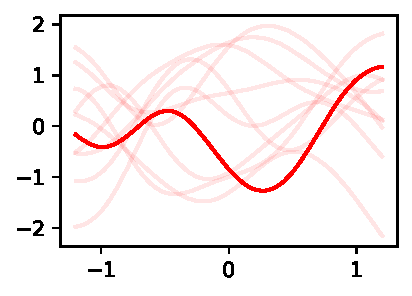
\includegraphics[width=\textwidth]{exponentiated_kernel.pdf}
        \subcaption{Squared Exponential Kernel}
        \label{fig:squared_exp}
    \end{subfigure}%
    \caption[
        Gaussian process realisations with Mat\'ern and squared exponential
        kernels
    ]{
        Ten sample realisations from 4 different kernels, with one realisation
        bolded.
        Samples
        for each kernel were generated from the same seed and the
        hyperparameters $\ell,$ and $\sigma_k$ were set to 1.
    }
    \label{fig:kernels}
\end{figure}

Realisations from zero-mean Gaussian processes with this kernel are
$\lfloor\nu\rfloor$ times mean square differentiable
\parencite{rasmussen_gaussian_2008}.
The most common values for $\nu$ are $1/2, 3/2$ and $5/2,$ which result in
functions that are 0, 1, and 2 times mean square differentiable. In these cases
the kernel can be slightly simplified to:
$$
    k_{1/2}(x, x^\prime)
    = \sigma^2_k\exp\left(-\frac{||x - x^\prime||}{\ell}\right),
$$
$$
    k_{3/2}(x, x^\prime)
    = \sigma^2_k
    \left(1 + \frac{\sqrt{3}||x - x^\prime||}{\ell}\right)
    \exp\left(-\frac{\sqrt{3}||x - x^\prime||}{\ell}\right),
$$
and
$$
    k_{5/2}(x, x^\prime)
    = \sigma^2_k
    \left(
    1 + \frac{\sqrt{5}||x - x^\prime||}{\ell} + \frac{5||x - x^\prime||}{3\ell^2}
    \right)
    \exp\left(-\frac{||x - x^\prime||^2}{2*\ell^2}\right).
$$
The increasing smoothness of these kernels can be see in Figures
\ref{fig:mat_one_half}, \ref{fig:mat_three_halves},
and \ref{fig:mat_five_halves}.

Zero-mean Gaussian processes with a Mat\'ern kernel are $n$ times mean square
differentiable, for all $n < \nu.$ As seen in Figure \ref{fig:kernels}, this
means that this kernel allows for flexibility in how smooth realised functions
are.

\subsubsection*{Squared Exponential Kernel}

As $\nu\to\infty,$ the Mat\'ern kernel converges to a kernel which we call
the squared exponential
kernel \parencite[85]{rasmussen_gaussian_2008}.

\begin{definition}[Squared Exponential Kernel]
    The \bemph{squared exponential kernel} is a covariance kernel with the form
    $$
        k(x, x^\prime)
        = \sigma^2_k\exp\left(-\frac{||x - x^\prime||^2}{2\ell^2}\right).
    $$ $\sigma^2_k$ and $\ell$ are hyperparameters.
\end{definition}

By construction, the squared exponential kernel is infinitely
mean square differentiable, which can visually be seen in \ref{fig:squared_exp}.
Despite this being the `default' kernel in much of
the literature (for example \cite{gutmann_bayesian_2016}), infinite
differentiability is a very strong condition that may not be appropriate in
all circumstances.

% Both the Mat\'ern and squared exponential kernels depend only on 
% $||x - x^\prime||,$ (they are stationary kernels).

\subsubsection*{Length and Amplitude Hyperparameters}

\begin{figure}[htbp]
    \centering
    \begin{subfigure}[b]{0.5\textwidth}
        \centering
        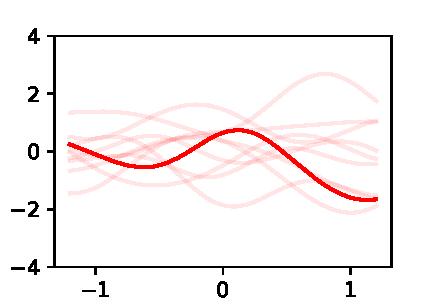
\includegraphics[width=\textwidth]{GP_ell_5_sigma2_5_tenths.pdf}
        \subcaption{$\ell = \sigma^2_k = 1/2$}
        \label{fig:half_half}
    \end{subfigure}%
    \hfill%
    \begin{subfigure}[b]{0.5\textwidth}
        \centering
        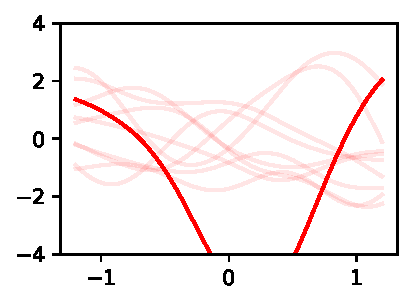
\includegraphics[width=\textwidth]{GP_ell_5_sigma2_20_tenths.pdf}
        \subcaption{$\ell = 1/2, \sigma^2_k = 2$}
        \label{fig:half_two}
    \end{subfigure}
    \begin{subfigure}[b]{0.5\textwidth}
        \centering
        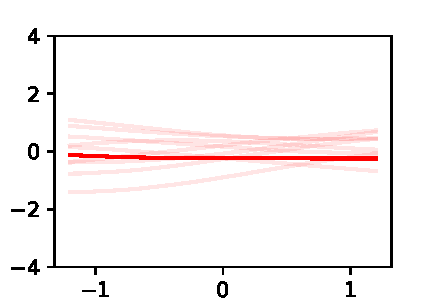
\includegraphics[width=\textwidth]{GP_ell_20_sigma2_5_tenths.pdf}
        \subcaption{$\ell = 2, \sigma^2_k = 1/2$}
        \label{fig:two_half}
    \end{subfigure}%
    \hfill%
    \begin{subfigure}[b]{0.5\textwidth}
        \centering
        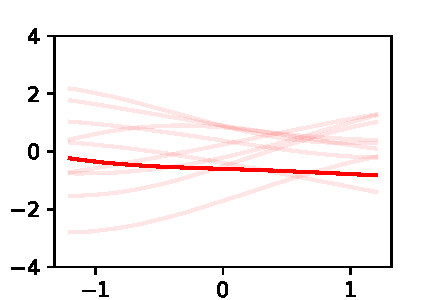
\includegraphics[width=\textwidth]{GP_ell_20_sigma2_20_tenths.pdf}
        \subcaption{$\ell = \sigma^2_k = 2$}
        \label{fig:two_two}
    \end{subfigure}%
    \caption[{
        Gaussian process realisations with differing length and scale
        hyperparameters in a squared exponential kernel.
    }]{
        Ten realisations of zero-mean Gaussian processes with the squared
        exponential kernel, varying the length and amplitude parameters.
        The samples were generated using the same seed
    }
    \label{fig:length_amp}
\end{figure}

In both the Mat\'ern and squared exponential kernels
(as well as most other common kernel choices), there are two
hyperparameters $\ell$ and $\sigma^2_k,$ which are referred to as length and
amplitude hyperparameters. $\ell$ determines how close two points need
to be to be highly correlated. Larger values of $\ell$ generates functions with
higher correlation within a larger neighbourhood,
as seen in Figure \ref{fig:length_amp}. $\sigma^2_k$ does not impact
the correlation between $x$ and $x^\prime,$ but scales the correlation
matrix. In other words, larger $\sigma^2_k$ increases the size but not the rate of
fluctuations. This can be seen comparing Figure \ref{fig:half_half} to Figure
\ref{fig:half_two}.

Other kernels exist and are used in the literature. Here we briefly discuss when
$k(x, x^\prime)$ is a valid kernel. We need the formal notions of symmetry and
positive semi-definite.

\begin{definition}[Symmetric]\label{def:sym_mat}
    A (square) matrix $\mathbf{A}$ is \bemph{symmetric} if $A = A^T.$
\end{definition}

\begin{definition}[Positive Semi-Definite]\label{def:pos_def_mat}
    An $n\times n$ matrix $\mathbf{A}$ is \bemph{positive semi-definite} if
    $\mathbf{v}^T\mathbf{A}\mathbf{v} \geq 0$ for all $\mathbf{v}\in\R^n.$
\end{definition}

\begin{theorem}
    Any kernel $k$ is admissible if the gram matrix
    $$\mathbf{K} = \begin{bmatrix}
            k(x_1, x_1) & k(x_1, x_2) & \dots  & k(x_1, x_n) \\
            k(x_2, x_1) & \ddots      &        & \vdots      \\
            \vdots      &             & \ddots & \vdots      \\
            k(x_n, x_1) & \cdots      & \cdots & k(x_n, x_n)
        \end{bmatrix}$$ associated with $k$ is symmetric and positive
    semi-definite for all choices of $(x_1, \dots, x_n),$ for finite $n.$
\end{theorem}
\begin{theorem}
    The Mat\'ern kernel and squared exponential kernels are admissible.
\end{theorem}
\begin{proof}
    The proof of the above two theorems are beyond the scope of this thesis,
    and involves analysis of spectral densities.
    See \cite[chapter 4]{rasmussen_gaussian_2008} for more details.
\end{proof}

\section{Gaussian Process Regression}

Given a realisation of a Gaussian process $f$, observed at the set of indices
$\bx^\ast,$ we can make inferences on unobserved indices $\bx$ by considering the
Gaussian process conditioned on $f(\bx^\ast).$
Since $f$ is a realisation of a Gaussian
process, the distribution of $f(\bx) | f(\bx^\ast)$ reduces to linear algebra
and has a multivariate normal distribution.

\begin{theorem}[Conditional Multivariate Normal Distribution is Multivariate Normal]
    \label{thm:cond_mvn}
    If
    $$
        \begin{bmatrix}
            f(\bx) \\
            f(\bx^\ast)
        \end{bmatrix} \sim \MVN\left(
        \begin{bmatrix}
                m(\bx) \\
                m(\bx^\ast)
            \end{bmatrix}, \begin{bmatrix}
                K            & K^{*}  \\
                (K^{\ast})^T & K^{**}
            \end{bmatrix}
        \right),
    $$
    then
    $$
        f(\bx) | f(\bx^\ast)
        \sim \MVN\left(
        m(\bx) + K^{*}(K^{**})^{-1}(f(\bx^\ast) - m(\bx^\ast)), \,\,
        K - K^{\ast}(K^{**})^{-1}(K^{\ast})^T
        \right).
    $$
\end{theorem}
\begin{proof}
    % https://statproofbook.github.io/P/mvn-cond.html
    Since marginal distribution of the multivariate normal distribution, is also
    multivariate normal,
    $f(\bx^\ast) \sim \MVN(m(\bx^\ast), K).$
    Let the inverse of $\begin{bmatrix}
            K            & K^{*}  \\
            (K^{\ast})^T & K^{**}
        \end{bmatrix}$ be
    $$
        \begin{bmatrix}
            \tilde{K}            & \tilde{K}^{\ast} \\
            (\tilde{K}^{\ast})^T & \tilde{K}^{**}
        \end{bmatrix}
    $$
    where

    \begin{align*}
        \tilde{K}
        := & (K - K^{\ast} (K^{**})^{-1} (K^{\ast})^T)^{-1}  \\
        \tilde{K}^{\ast}
        := & -(K - K^{\ast} (K^{**})^{-1} (K^{\ast})^T)^{-1}
        K^{\ast} (K^{**})^{-1}                               \\
        \tilde{K}^{**}
        := & (K^{**})^{-1} + (K^{**})^{-1} (K^{\ast})^T (K
        - K^{\ast} (K^{**})^{-1} (K^{\ast})^T)^{-1} K^{\ast} (K^{**})^{-1}
    \end{align*}
    by the inverse of a block matrix. Therefore
    \begin{align*}
        p(f(\bx) | f(\bx^\ast))
        =       & \frac{p(f(\bx), f(\bx^\ast))}{p(f(\bx^\ast))}        \\
        \propto & \frac{\exp \left[ -\frac{1}{2} \left(\begin{bmatrix}
                                                               f(\bx) \\
                                                               f(\bx^\ast)
                                                           \end{bmatrix} -
        \begin{bmatrix}
                m(\bx) \\
                m(\bx^\ast)
            \end{bmatrix}
        \right)^\mathrm{T} \begin{bmatrix}
                               K            & K^{\ast} \\
                               (K^{\ast})^T & K
                           \end{bmatrix}^{-1} \left(
        \begin{bmatrix}
                f(\bx) \\
                f(\bx^\ast)
            \end{bmatrix}-
        \begin{bmatrix}
                m(\bx) \\
                m(\bx^\ast)
            \end{bmatrix}\right) \right]}
        {
        \exp \left[
        -\frac{1}{2}
        (f(\bx^\ast)-m(\bx^\ast))^\mathrm{T}
        (K^{**})^{-1}
        (f(\bx^\ast)-m(\bx^\ast))
        \right]
        }                                                              \\
        =       & \exp \left[ -\frac{1}{2} \left(\begin{bmatrix}
                                                         f(\bx) \\
                                                         f(\bx^\ast)
                                                     \end{bmatrix} -
        \begin{bmatrix}
                m(\bx) \\
                m(\bx^\ast)
            \end{bmatrix}
        \right)^\mathrm{T} \begin{bmatrix}
                               K            & K^{\ast} \\
                               (K^{\ast})^T & K^{**}
                           \end{bmatrix}^{-1} \left(
        \begin{bmatrix}
                f(\bx) \\
                f(\bx^\ast)
            \end{bmatrix} -
        \begin{bmatrix}
                m(\bx) \\
                m(\bx^\ast)
            \end{bmatrix} \right)\right.                                   \\
                & \hphantom{\exp \left[\right.} \left.
        + \frac{1}{2}(f(\bx^\ast)-m(\bx^\ast))^\mathrm{T}
        (K^{**})^{-1}
        (f(\bx^\ast)-m(\bx^\ast))\right]                               \\
        =       & \exp \left[
        -\frac{1}{2} \left(
        (f(\bx)-m(\bx))^\mathrm{T}
        \tilde{K}
        (f(\bx)-m(\bx))\right.\right.                                  \\
                & \hphantom{\exp \left[
        -\frac{1}{2} \left( \right.\right.}
        + 2 (f(\bx)-m(\bx))^\mathrm{T}
        \tilde{K}^{\ast}
        (f(\bx^\ast)-m(\bx^\ast))                                      \\
                & \hphantom{\exp \left[
        -\frac{1}{2} \left( \right.\right.}
        \left.
        + (f(\bx^\ast)-m(\bx^\ast))^\mathrm{T}
        \tilde{K}^{**}
        (f(\bx^\ast)-m(\bx^\ast))
        \right)
        \\
                & \hphantom{\exp \left[
        -\frac{1}{2} \left( \right.\right.}\left.
        + \frac{1}{2} (f(\bx^\ast)-m(\bx^\ast))^\mathrm{T}
        (K^{**})^{-1}
        (f(\bx^\ast)-m(\bx^\ast))
        \right]                                                        \\
        \propto & \exp \left[
        -\frac{1}{2}
        (f(\bx)-m(\bx))^\mathrm{T}
        \tilde{K}
        (f(\bx)-m(\bx))\right.                                         \\
                & \hphantom{\exp \left[
        -\frac{1}{2} \left( \right.\right.}
        -\left.
        (f(\bx)-m(\bx))^\mathrm{T}
        \tilde{K}^{\ast}
        (f(\bx^\ast)-m(\bx^\ast))
        \right] \tag{by removing the terms independent of $f(\bx)$}.
    \end{align*}
    Since
    $$
        p(\mathbf{z})
        \propto \exp\left(
        -\frac{1}{2}\mathbf{z}^T\Sigma^{-1}\mathbf{z}
        + \mathbf{z}^T\mathbf{c}
        \right)
        \implies \mathbf{z} \sim \MVN\left(\Sigma \mathbf{c}, \Sigma\right),
    $$
    $f(\bx) - m(\bx) | f(\bx^\ast)$ is
    multivariate normal with mean
    \begin{align*}
        - \tilde{K}^{-1}\tilde{K}^{\ast}(f(\bx^\ast) - m(\bx^\ast))
        = & (K - K^{\ast} (K^{**})^{-1} (K^{\ast})^T)                                   \\
          & \times(K - K^{\ast} (K^{**})^{-1} (K^{\ast})^T)^{-1} K^{\ast} (K^{**})^{-1}
        (f(\bx^\ast) - m(\bx^\ast))                                                     \\
        = & K^{\ast} (K^{**})^{-1}(f(\bx^\ast) - m(\bx^\ast))
    \end{align*}
    and covariance matrix
    $$
        \tilde{K}^{-1} = K - K^{\ast} (K^{**})^{-1} (K^{\ast})^T
    $$
    by the alternative parameterisation of the multivariate normal distribution
    as a member of the exponential family of distributions
    (see \cite[Table of Distributions]{noauthor_exponential_2024}).
    Finally, by the linearity of the multivariate normal mean,
    $$
        f(\bx) | f(\bx^\ast)
        \sim \MVN\left(
        m(\bx) + K^{\ast}(K^{**})^{-1}(f(\bx^\ast) - m(\bx^\ast)), \,\,
        K - K^{\ast}(K^{**})^{-1}(K^{\ast})^T
        \right).
    $$
\end{proof}

\begin{figure}[htbp]
    \centering
    \begin{subfigure}[b]{0.5\textwidth}
        \centering
        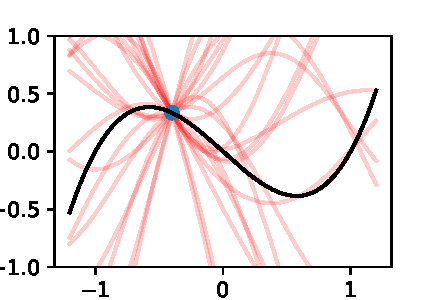
\includegraphics[width=\textwidth]{cub_GP_1_iters.pdf}
    \end{subfigure}%
    \hfill%
    \begin{subfigure}[b]{0.5\textwidth}
        \centering
        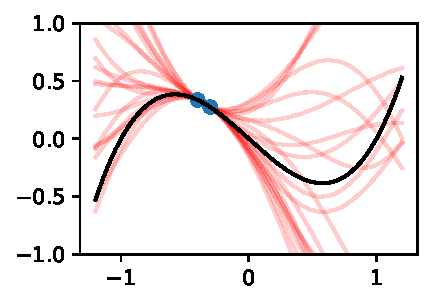
\includegraphics[width=\textwidth]{cub_GP_2_iters.pdf}
    \end{subfigure}
    \begin{subfigure}[b]{0.5\textwidth}
        \centering
        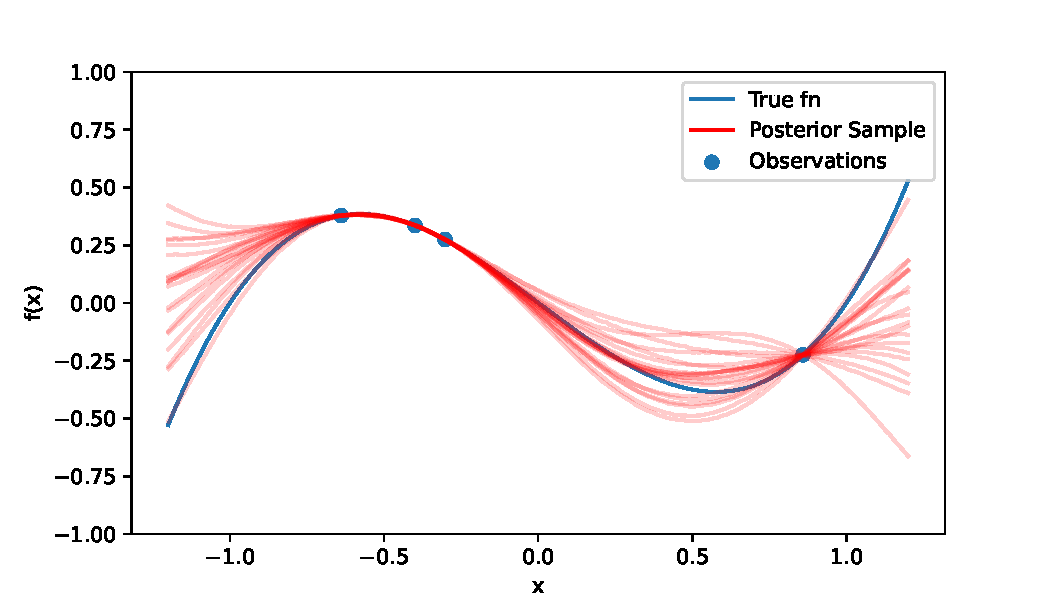
\includegraphics[width=\textwidth]{cub_GP_4_iters.pdf}
    \end{subfigure}%
    \hfill%
    \begin{subfigure}[b]{0.5\textwidth}
        \centering
        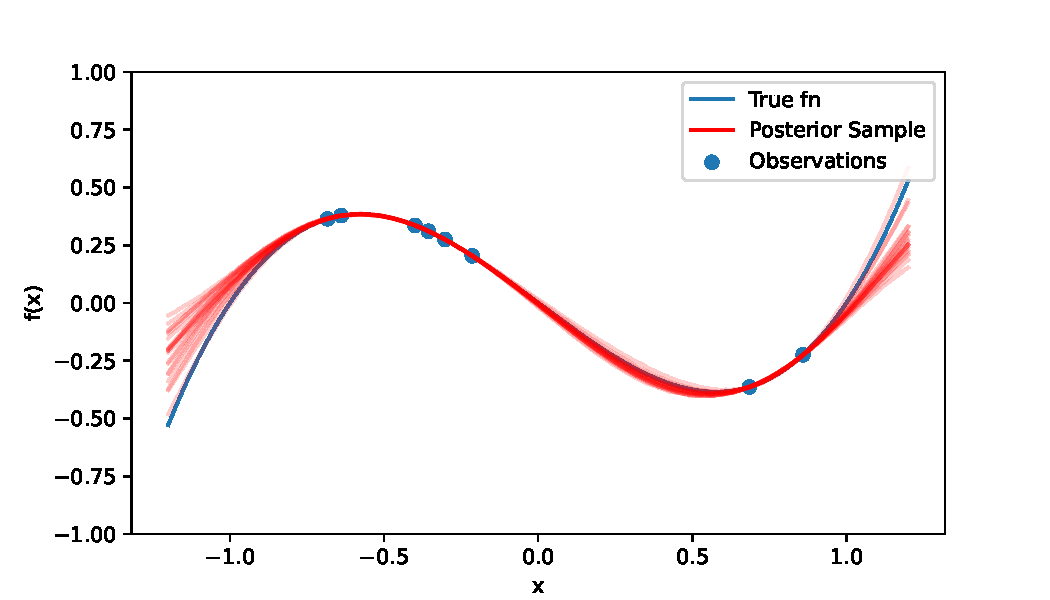
\includegraphics[width=\textwidth]{cub_GP_8_iters.pdf}
    \end{subfigure}%
    \caption[{
        Gaussian process regression without noise
    }]{
        Sequence of Gaussian process regressions on the target function
        (black) $f(x) = x(x-1)(x+1),$ after 1, 2, 4, and 8 observations in
        blue. The red lines are new realisations from the conditioned Gaussian
        process. The Gaussian process was zero-mean and had a squared
        exponential kernel. The hyperparameters were fixed with $\ell = 2.7$
        and $\sigma^2_k = 1.1.$
    }
    \label{fig:no_var_cub_reg}
\end{figure}

We can use this to fit a Gaussian process to set of indices $\bx^\ast$ with
observations $f(\bx^\ast).$
This can be used in an iterative process where $f(x)$
may be expensive to compute and by treating $f$ as a Gaussian process
realisation, the function can be probabilistically interpolated for unobserved
$f(x).$ Figure \ref{fig:no_var_cub_reg} empirically demonstrates that as
the number of points that the Gaussian process is conditioned on increases,
the variance in the sample paths decreases.

\subsection*{Observation Variance}

For most functions, model outputs, or processes desirable for
approximating through Gaussian process regression, it may not be possible to
observe $f(\bx)$ directly, but observations may be noisy.
The simplest assumption is that the
observations are of the form
$$
    f_o(\bx^\ast) = f(\bx^\ast) + \bm{\varepsilon}
$$
where $\bm{\varepsilon} \sim \MVN(\mathbf{0}, \sigma^2_o I).$
Under these assumptions,
$\mathrm{Cov}(f_o(\bx^\ast), f_o(\bx^\ast)) = K^{**} + \sigma^2_o I,$
where $K^{**} = \mathrm{Cov}(f(\bx^\ast), f(\bx^\ast))$
matrix of $f(\bx^\ast)$ without noise. Therefore the conditional
distribution of our unobserved function outputs given noisy observations
$$
    f(\bx) | f_o(\bx^\ast)
    \sim \MVN\left(
    m(\bx) + K^{\ast}
    (K^{**} + \sigma^2_o I)^{-1}
    (f(\bx^\ast) - m(\bx^\ast)), \,\,
    K - K^{\ast}(K^{**} + \sigma^2_o I)^{-1}(K^{\ast})^T
    \right).
$$


\begin{figure}[htbp]
    \centering
    \begin{subfigure}[b]{0.5\textwidth}
        \centering
        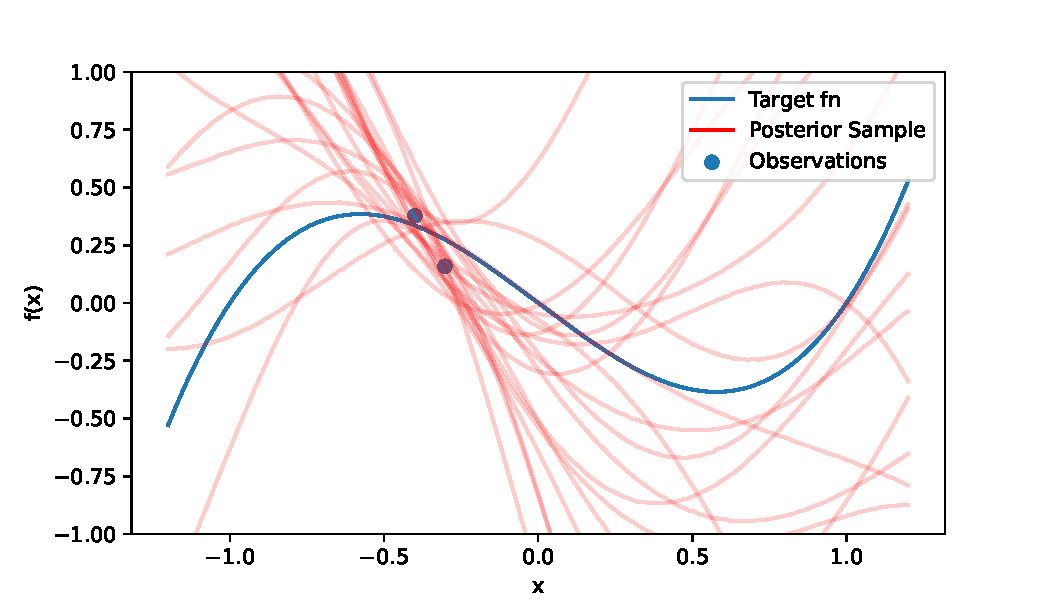
\includegraphics[width=\textwidth]{cub_GP_err_2_iters.pdf}
    \end{subfigure}%
    \hfill%
    \begin{subfigure}[b]{0.5\textwidth}
        \centering
        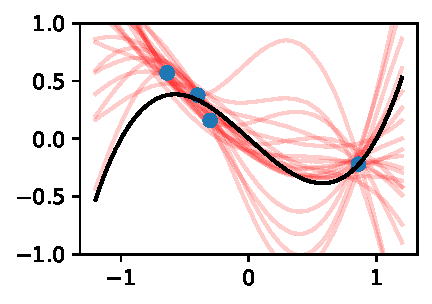
\includegraphics[width=\textwidth]{cub_GP_err_4_iters.pdf}
    \end{subfigure}
    \begin{subfigure}[b]{0.5\textwidth}
        \centering
        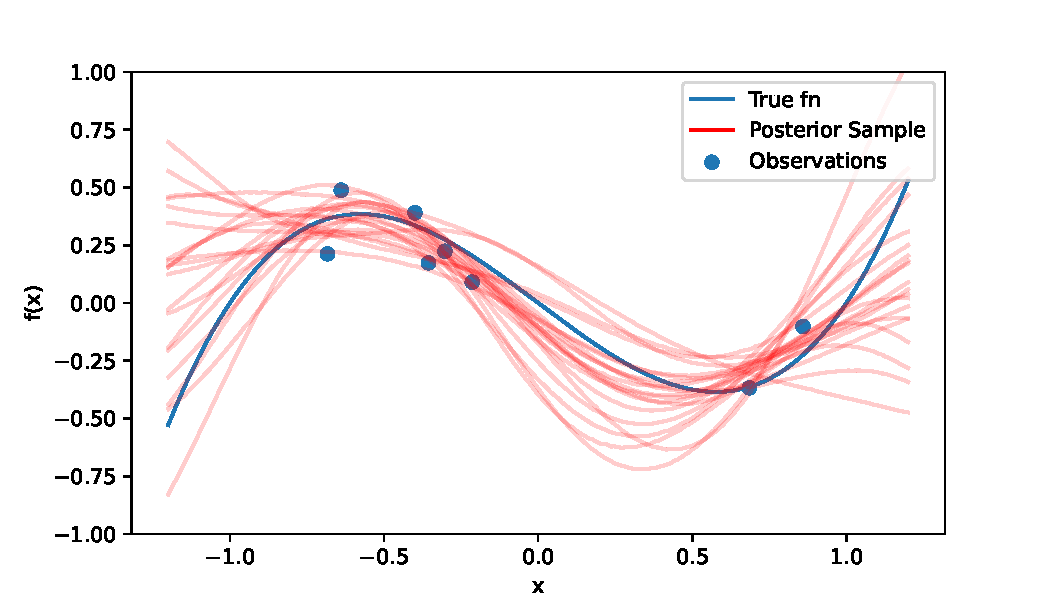
\includegraphics[width=\textwidth]{cub_GP_err_8_iters.pdf}
    \end{subfigure}%
    \hfill%
    \begin{subfigure}[b]{0.5\textwidth}
        \centering
        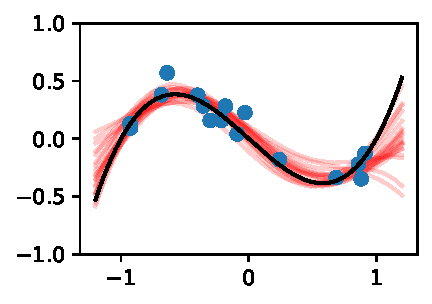
\includegraphics[width=\textwidth]{cub_GP_err_16_iters.pdf}
    \end{subfigure}%
    \caption[{
        Gaussian process regression with noise
    }]{
        Sequence of Gaussian process regressions on the target function
        (black) $f(x) = x(x-1)(x+1),$ after 2, 4, 8, and 16 observations of
        $f(x_i) + \varepsilon_i,$ where $\varepsilon_i$ is i.i.d.\
        $\MVN(0, \sigma^2_o)$ with $\sigma^2_o = 0.01$
        in blue. The red lines are new realisations from the conditioned
        Gaussian process. The Gaussian process was 0 mean and had a squared
        exponential kernel. The hyperparameters were fixed with $\ell = 2.7$
        and $\sigma^2_k = 1.1.$
    }
    \label{fig:var_cub_reg}
\end{figure}

The observations $f_o(\bx^\ast)$ contain less information than when $f(\bx^\ast)$
is directly observed, and hence interpolating to $\bx$ or even $\bx^\ast$
naturally has a
greater degree of uncertainty as seen in Figure \ref{fig:var_cub_reg}.

\section{Model Selection}

After deciding to use a Gaussian process to approximate a function, there is
still a variety of choices that need to be made, particularly
regarding the covariance kernel. The first
choice needs to be the class of kernel used.

\subsection*{Kernel}

The appropriate choice of kernel will depend on the properties of the
target function $f$ to be regressed to. In the case of estimating an extremely
stochastic distribution (such as the price of a stock over time), a
kernel with a high degree of mean square differentiability would be
inappropriate. On the other hand a Mat\'ern 1/2 kernel may be appropriate,
since it is not mean square differentiable. If it is known that the target
function is smooth, such as a polynomial function or $\sin(x)$,
then the choice of squared
exponential kernel is the most appropriate kernel.

\subsection*{Hyperparameters}

The kernel hyperparameters $\ell$ and $\sigma^2_k$ are generally not fixed
\emph{a priori}. Similarly, the observation variance $\sigma^2_o$
may not be known.
There are two main (frequentist) ways to fit these hyperparameters:
maximum likelihood estimation, and leave-one-out cross validation.

Defining the likelihood
$
    \mathcal{L}(\ell, \sigma^2_k, \sigma^2_o)
    := p(f(\bx^\ast) | \ell, \sigma^2_k, \sigma^2_o)
$ in the usual way,
the maximum likelihood estimates are
\begin{align}
    \{\hat{\ell}, \hat{\sigma}^2_k, \hat{\sigma}^2_o\} :=
    \argmax_{\{\ell, \sigma^2_k, \sigma^2_o\}}
    \mathcal{L}(\ell, \sigma^2_k, \sigma^2_o)
    \label{eq:MLE_GP}
\end{align}
which is equivalent to minimising
$$
    -\ln(\mathcal{L}) =\frac{1}{2} \left[
    \ln (|K^{**}(\ell, \sigma^2_k) + \sigma^2_o|\,)
    + (f(\bx^\ast) - m(\bx^\ast))^T
    (K^{**}(\ell, \sigma^2_k) + \sigma^2_o)^{-1}
    (f(\bx^\ast) - m(\bx^\ast)) + c
    \right].
$$
The covariance matrix generated by the choice of kernel $K^{**}$ is
explicitly written with its dependence on $\ell$ and $\sigma^2_k.$ Here $c$ is a
constant.

Leave-one-out cross validation aims to maximise the predictive log
probability:
\begin{align}
    \{\tilde{\ell}, \tilde{\sigma}^2_k, \tilde{\sigma}^2_o\}
    := \argmax_{\ell, \sigma^2_k, \sigma^2_o} \sum_{i}
    \ln p(f_i(\bx^\ast) | f_{-i}(\bx^\ast), \ell, \sigma^2_k, \sigma^2_o),
    \label{eq:pred_log_prob}
\end{align}
where $f_i(\bx^\ast) | f_{-i}(\bx^\ast)$ is the distribution of the
$i$th element of $f(\bx^\ast)$ conditioned on the rest of the
observed data excluding that element (represented by $f_{-i}(\bx^\ast)$).
$f_i(\bx^\ast) | f_{-i}(\bx^\ast)$ can be found by
Theorem \ref{thm:cond_mvn}. Computationally efficient methods for calculating
the predictive log probability (Equation \ref{eq:pred_log_prob})
that avoid having to invert the covariance
matrix for every summand element exist. In particular it can be shown that
$f_i(\bx^\ast) | f_{-i}(\bx^\ast)$ has mean
$$
    f_i(\bx^\ast) - m_i(\bx^\ast)
    - [(K^{**} + \sigma^2_o I)^{-1}(f(\bx^\ast) - m(\bx^\ast))]_i
    /[(K^{**} + \sigma^2_o I)^{-1}]_{ii}
$$
and variance $1/[(K^{**} + \sigma^2_o I)^{-1}]_{ii},$ where both the mean and
covariance are (surprisingly) independent of $f_i(\bx^\ast)$
\parencite[116]{rasmussen_gaussian_2008}.

Recent work has shown that at least under specific conditions, the
leave-one-out estimates for the scale hyperparameter are more robust to a larger
family of target functions \parencite{naslidnyk_comparing_2024}, and the
broader literature seems to favor leave-one-out cross validation (for example
see \cite{gutmann_bayesian_2016}).

Finally there is scope for a Bayesian approach to model selection. By setting
priors on the hyperparameters (sometimes called hyper-priors)
and using the likelihood as described
in the maximum likelihood estimation approach (Equation \ref{eq:MLE_GP}),
a posterior distribution can be
contrived. Samples could then be taken from the posterior density
of the hyperparameters. Alternatively a point estimate could be drawn by
choosing the maximum a posteriori estimate (i.e. the mode of the
posterior density). Posterior
samples of the hyperparameters, can then capture some of the model fit
uncertainty, unlike in a point estimate.

\subsection*{Mean Functions}

Although in the majority of use cases for Gaussian processes, the mean function
is assumed to be zero, it is not necessary for this to be the case. In cases
where the discrepancy function has been estimated by a Gaussian process,
the mean function has been assumed to be quadratic, such as in
\parencite{gutmann_bayesian_2016}. Gaussian process regression is relatively
resilient to misspecified mean function in areas with samples. 
However, the regression will return to
the behaviour of the mean function where there are no points to regress to.

\begin{figure}[htbp]
    \centering
    \begin{subfigure}[b]{0.5\textwidth}
        \centering
        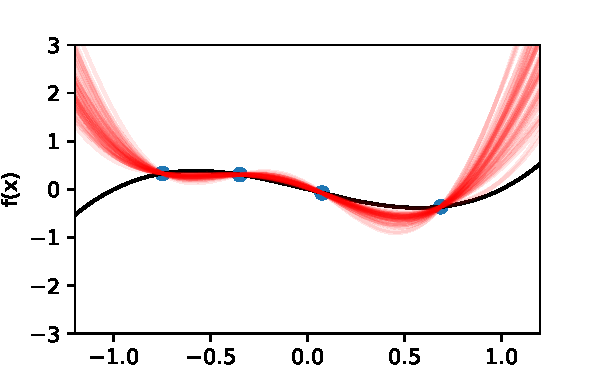
\includegraphics[width=\textwidth]{positive_quad_mean_GP.pdf}
    \end{subfigure}%
    \hfill%
    \begin{subfigure}[b]{0.5\textwidth}
        \centering
        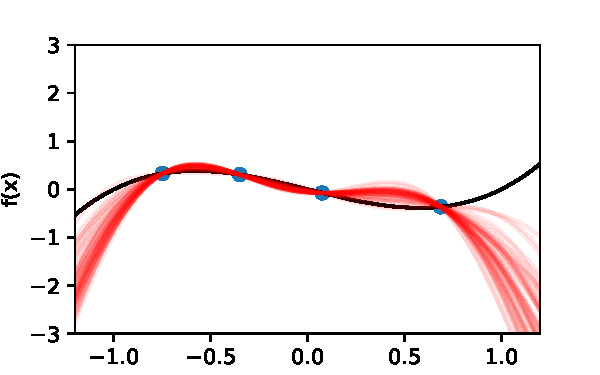
\includegraphics[width=\textwidth]{negative_quad_mean_GP.pdf}
    \end{subfigure}
    \caption[
        The effect of the mean function on Gaussian processes
    ]{Gaussian process regressions on the target function (black) 
    $f(x) = x(x -1)(x+1)$, 4, observations of $f(x_i)$ in blue. The left
    Gaussian process had mean function $3x^2,$ and the right Gaussian process
    had mean function $-3x^2.$
    The red lines are new realisations from the conditioned Gaussian process.}
    \label{fig:means}
\end{figure}

This can be seen in Figure \ref{fig:means}. Around the observed data in blue,
the processes have similar predictions for the function, however
outside of where the function has
been observed, both
Gaussian processes return to their quadratic mean functions.
Specifying a mean for the Gaussian process may be appropriate, but it must
be done with caution.

\section{Bayesian Acquisition Functions}

Gaussian processes may be a useful approximation of $\E[\D(\btheta)].$ We can
express the Gaussian process surrogate model as $\D_\GP(\btheta),$ trained on
samples of $\D(\btheta).$
Considering the approximate Bayesian computation described in
Algorithm \ref{alg:abc}, samples are only accepted when $\D(\btheta)$ is small.
Therefore we care most about accurately approximating $\D(\btheta)$ where
$\E[\D(\btheta)]$ is small since the probability of acceptance elsewhere is
negligible. Therefore we focus our model sampling where we predict the Gaussian
process is small, or where the variance of the Gaussian process is large
(hence the true values are highly uncertain), to avoid unnecessary model runs
that may be extremely time-consuming.

These ideas are
formalised by Bayesian acquisition functions $\A(\btheta)$ which
describe the desirability of sampling from $\btheta$ as a combination of low
posterior mean and uncertainty.

\subsection*{Lower Confidence Bound}

The lower confidence bound acquisition function is a calculation of the lower
bound of the confidence interval of the regressed Gaussian process. It is a
function of both the posterior mean and variance, weighted according to a
constant $\eta.$

\begin{definition}[Lower Confidence Bound]
    The \bemph{lower confidence bound} of a Gaussian process $f$ at $x$ given
    some observations $\bx^\ast$ is
    $$
        \A_\mathrm{LCB}(x)
        := \E[f(x) | f(\bx^\ast)]
        - \eta \sqrt{\mathrm{Var}[f(x) | f(\bx^\ast)]}.
    $$
\end{definition}

For example, when $\eta = 1.96,$ $\A_\text{LCB}(x)$ returns the lower
bound of the 95\% confidence interval at $x.$ In problems where a global
minimum is to be estimated, and where $f$ is regressed on realisations of
a model, the next point to sample from the
model would then be chosen $\argmin_{x} A_\mathrm{LCB}(x).$
Larger $\eta$ will prioritise
exploration of the space of $x,$ whereas small $\eta$ will continue to sample
around areas of confirmed low mean.

$\eta$ can also be replaced by
$\eta(t),$ where $t$ is the number of points that have been regressed on.
Generally $\eta(t)$ is chosen to be an increasing function, so that exploration
is given more weight over time. Some theoretical results regarding optimal
choice of
$\eta(t)$ are given in \cite{srinivas_gaussian_2010}, and are highly dependent
on the choice of covariance function and dimensionality of the parameter space.

\subsection*{Probability of Improvement}

The probability of improvement is simply a measure of how probable it is that
an observation at $x$ is better than the previous best observation.

\begin{definition}
    The \bemph{probability of improvement} of a Gaussian process $f$ at $x$ given
    some observations $\bx^\ast$ is
    $$
        \A_\mathrm{PI}(x) := \Pr(f(x) < \mu^\ast),
    $$
    where $\mu^\ast := \min_{x^\ast\in\bx^\ast}f(x^\ast).$
\end{definition}

Unlike the lower confidence bound, we choose $\argmax_{x} A_\mathrm{PI}(x),$ as
the point which is most likely to better than our current best.

The probability of improvement can also be expressed as
$$
    \A_\mathrm{PI}(x) = \Pr(\min(f(x) - \mu^\ast, 0) < 0),
$$
which motivates the form of the next acquisition function.

\subsection*{Expected Improvement}

A similar acquisition function to the probability of improvement is the expected
improvement function. Rather than returning a the probability that $f(x)$ is
better (lower) than the current best, it also takes into account how large that
improvement is likely to be.

\begin{definition}
    The \bemph{expected improvement} of a Gaussian process $f$ at $x$ given
    some observations $\bx^\ast$ is
    $$
        \A_\EI(x)
        := \E[\min(f(x) - \mu^\ast, 0)],
    $$ where $\mu^\ast := \min_{x^\ast\in\bx^\ast}f(x^\ast).$
\end{definition}
The next point to be sampled from $\argmin_{x} A_\EI(x)$ is the point
where we expect $\mu^\ast$ to have the largest improvement, if it is indeed
improved.
\footnote{
    Bayesian acquisition functions are
    conventionally employed to find the maximum of an unknown function,
    and so generally, the expected improvement is maximised.
    However, in the context of $\D_\GP(\btheta),$ we want to find the minimum.
    Therefore we have reframed the expected improvement
    as a function to be minimised.
}
Both the probability of improvement and
expected improvement do not require a
choice of hyperparameter such as $\eta,$ but more exploration can be
encouraged by slightly altering the probability of improvement to
$\Pr(f(x) < \mu^\ast + \epsilon),$ and the expected improvement to
$\E[\min(f(x) - (\mu^\ast + \epsilon), 0)].$ $\epsilon$ allows for
new samples to be $\epsilon$ worse (larger) than the current best sample.
This is beneficial in the case where finding the exact global minimum may not
be the target, but rather exploring areas close to the minimum.



% $$\mu(\btheta) - \eta_t\sqrt{\mathrm{v}(\btheta)}$$
% with $\eta_t:= \sqrt{2\ln(\frac{t^{2d + 2}\pi^2}{3\varepsilon})},$ and
% $\varepsilon \in (0, 1)$ that can be chosen
% (with a lower epsilon resulting in more exploration), $\mu(\btheta)$ and
% $\mathrm{v}(\btheta)$ are the posterior mean and variance.
% $\varepsilon = 0.1$ was used.